\documentclass{oblivoir}
%%%Default packages
\usepackage{amsmath,amssymb,amsthm,kotex,tabu,graphicx,pifont}
\usepackage{../kswrapfig}

\usepackage{gensymb} %\degree

%%%More packages
%\usepackage{caption,subcaption}
%\usepackage[perpage]{footmisc}
%
\usepackage[skipabove=10pt,innertopmargin=10pt,nobreak=true]{mdframed}

\usepackage[inline]{enumitem}
\setlist[enumerate,1]{label=(\arabic*)}
\setlist[enumerate,2]{label=(\alph*)}

\usepackage{multicol}
\setlength{\columnsep}{30pt}
\setlength{\columnseprule}{1pt}
%
%\usepackage{forest}
%\usetikzlibrary{shapes.geometric,arrows.meta,calc}
%
%%%defi theo exam prob rema proo
%이 환경들 아래에 문단을 쓸 경우 살짝 들여쓰기가 되므로 \hspace{-.7em}가 필요할 수 있다.

\newcounter{num}
\newcommand{\defi}[1]
{\noindent\refstepcounter{num}\textbf{정의 \arabic{num})} #1\par\noindent}
\newcommand{\theo}[1]
{\noindent\refstepcounter{num}\textbf{정리 \arabic{num})} #1\par\noindent}
\newcommand{\revi}[1]
{\noindent\refstepcounter{num}\textbf{복습 \arabic{num})} #1\par\noindent}
\newcommand{\exam}[1]
{\bigskip\bigskip\noindent\refstepcounter{num}\textbf{예시 \arabic{num})} #1\par\noindent}
\newcommand{\prob}[1]
{\bigskip\bigskip\noindent\refstepcounter{num}\textbf{문제 \arabic{num})} #1\par\noindent}
\newcommand{\rema}[1]
{\bigskip\bigskip\noindent\refstepcounter{num}\textbf{참고 \arabic{num})} #1\par\noindent}
\newcommand{\proo}
{\bigskip\noindent\textsf{증명)}}

\newenvironment{talign}
 {\let\displaystyle\textstyle\align}
 {\endalign}
\newenvironment{talign*}
 {\let\displaystyle\textstyle\csname align*\endcsname}
 {\endalign}
%
%%%Commands

\newcommand{\procedure}[1]{\begin{mdframed}\vspace{#1\textheight}\end{mdframed}}

\newcommand\an[1]{\par\bigskip\noindent\textbf{문제 \ref{#1})}\par\noindent}

\newcommand\ann[2]{\par\bigskip\noindent\textbf{문제 \ref{#1})}\:\:#2\par\medskip\noindent}

\newcommand\ans[1]{\begin{flushright}\textbf{답 : }#1\end{flushright}}

\newcommand\anssec[1]{\bigskip\bigskip\noindent{\large\bfseries#1}}

\newcommand{\pb}[1]%\Phantom + fBox
{\fbox{\phantom{\ensuremath{#1}}}}

\newcommand\ba{\,|\,}

\newcommand\ovv[1]{\ensuremath{\overline{#1}}}
\newcommand\ov[2]{\ensuremath{\overline{#1#2}}}
%
%%%% Settings
%\let\oldsection\section
%
%\renewcommand\section{\clearpage\oldsection}
%
%\let\emph\textsf
%
%\renewcommand{\arraystretch}{1.5}
%
%%%% Footnotes
%\makeatletter
%\def\@fnsymbol#1{\ensuremath{\ifcase#1\or
%*\or **\or ***\or
%\star\or\star\star\or\star\star\star\or
%\dagger\or\dagger\dagger\or\dagger\dagger\dagger
%\else\@ctrerr\fi}}
%
%\renewcommand{\thefootnote}{\fnsymbol{footnote}}
%\makeatother
%
%\makeatletter
%\AtBeginEnvironment{mdframed}{%
%\def\@fnsymbol#1{\ensuremath{\ifcase#1\or
%*\or **\or ***\or
%\star\or\star\star\or\star\star\star\or
%\dagger\or\dagger\dagger\or\dagger\dagger\dagger
%\else\@ctrerr\fi}}%
%}   
%\renewcommand\thempfootnote{\fnsymbol{mpfootnote}}
%\makeatother
%
%%% 객관식 선지
\newcommand\one{\ding{172}}
\newcommand\two{\ding{173}}
\newcommand\three{\ding{174}}
\newcommand\four{\ding{175}}
\newcommand\five{\ding{176}}
\usepackage{tabto,pifont}
%\TabPositions{0.2\textwidth,0.4\textwidth,0.6\textwidth,0.8\textwidth}

\newcommand\taba[5]{\par\noindent
\one\:{#1}
\tabto{0.2\textwidth}\two\:\:{#2}
\tabto{0.4\textwidth}\three\:\:{#3}
\tabto{0.6\textwidth}\four\:\:{#4}
\tabto{0.8\textwidth}\five\:\:{#5}}

\newcommand\tabb[5]{\par\noindent
\one\:{#1}
\tabto{0.33\textwidth}\two\:\:{#2}
\tabto{0.67\textwidth}\three\:\:{#3}\medskip\par\noindent
\four\:\:{#4}
\tabto{0.33\textwidth}\five\:\:{#5}}

\newcommand\tabc[5]{\par\noindent
\one\:{#1}
\tabto{0.5\textwidth}\two\:\:{#2}\medskip\par\noindent
\three\:\:{#3}
\tabto{0.5\textwidth}\four\:\:{#4}\medskip\par\noindent
\five\:\:{#5}}

\newcommand\tabd[5]{\par\noindent
\one\:{#1}\medskip\par\noindent
\two\:\:{#2}\medskip\par\noindent
\three\:\:{#3}\medskip\par\noindent
\four\:\:{#4}\medskip\par\noindent
\five\:\:{#5}}
%
%%%% fonts
%
%\usepackage{fontspec, xunicode, xltxtra}
%\setmainfont[]{은 바탕}
%\setsansfont[]{은 돋움}
%\setmonofont[]{은 바탕}
%\XeTeXlinebreaklocale "ko"
%%%%
\begin{document}

\title{수학 : 02 이차방정식}
\author{}
\date{\today}
\maketitle
\tableofcontents
\newpage

%%%
\section{복소수}

%%
\subsection{허수와 복소수}

%
\exam{}
\begin{enumerate}
\item
이차방정식 \(x^2=4\)의 근은 \(x=2\), \(x=-2\)이다.
\item
이차방정식 \(x^2=0\)의 근은 \(x=0\)이다.
\item
이차방정식 \(x^2=-1\)의 근은 실수 중에서는 없다.
\(x\)가 실수이면 \(x^2\ge0\)이기 때문이다.
이런 형식의 이차방정식의 근을 이야기하기 위해 실수가 아닌 새로운 수 \(i\)를 도입한다.
\end{enumerate}

%
\begin{mdframed}
\defi{}
제곱해서 \(-1\)이 되는 새로운 수를 생각하여 이것을 기호 \(i\)로 나타낸다.
즉
\[i^2=-1\]
이다.
\end{mdframed}
따라서 \(i\)는 방정식 \(x^2=-1\)의 근이 된다.
한편 \(-i\)도 \((-i)^2=i^2=-1\)로 계산한다고 생각하여, \(-i\)도 근이 된다.
즉 이차방정식 \(x^2=-1\)의 근은 \(\pm i\)이다.

%
\exam{}
\begin{enumerate}\label{comp1}
\item
이차방정식 \(x^2=-4\)을 변형하면
\[\left(\frac x2\right)^2=-1\]
이다.
따라서 \(\frac x2=\pm i\)이고 \(x=\pm2i\)이다.
\item
이차방정식 \(x^2-2x+2=0\)을 변형하면
\[(x-1)^2=-1\]
이다.
따라서 \(x-1=\pm i\)이고 \(x=1\pm i\)이다.
\end{enumerate}

%
\prob{다음 이차방정식의 해를 구하여라.}
\begin{enumerate}\label{comp2}
\item
\(x^2=-3\)
\item
\(4x^2=-1\)
\item
\(x^2+6x+10=0\)
\end{enumerate}

\bigskip
예시 \ref{comp1}의 (2)\와 문제 \ref{comp2}의 (3)에서의 답처럼 \(a+bi\)형식의 수를 \emph{복소수}라고 한다.

%
\begin{mdframed}
\defi{복소수}
\(a\), \(b\)가 실수일 때, \(a+bi\)로 표현되는 수를 \emph{복소수}라고 한다.
이때 \(a\)를 \emph{실수부분}, \(b\)를 \emph{허수부분}이라고 한다.
\end{mdframed}

%
\exam{\(z=a+bi\)라고 할 때,}
\begin{enumerate}
\item
\(b=0\)이면 \(z=a\)\가 되어 \(z\)는 실수이다.
\item
\(b\neq0\)이면 \(z\)는 실수가 아니다.
이처럼 실수가 아닌 복소수를 \emph{허수}라고 한다.
\item
\(a=0\), \(b\neq0\)이면 \(z=bi\)이다.
이처럼 실수부분이 없는 허수를 \emph{순허수}라고 한다.
\end{enumerate}

%
\prob{}\label{comp3}
다음 복소수들 중 실수의 개수를 \(x\), 허수의 개수를 \(y\), 순허수의 개수를 \(z\)라고 할 때, \(x\), \(y\), \(z\)의 값을 각각 구하여라.
\begin{mdframed}[innertopmargin=0pt,leftmargin=60pt,rightmargin=60pt]
\[2+\sqrt2i,\qquad\sqrt3-i,\qquad5i,\qquad-\pi\]
\end{mdframed}
\bigskip

%
\prob{다음 중 옳지 않은 것은?}\label{comp4}
\par\vspace{-20pt}
\tabd
{허수는 복소수이다.}
{\(2-\sqrt5i\)의 실수부분은 \(2\), 허수부분은 \(-\sqrt5\)이다.}
{\(2\)의 허수부분은 \(0\)이다.}
{\(0\)은 허수이다.}
{\(-3i\)는 순허수이다.}

%
\begin{mdframed}
\defi{두 복소수가 서로 같을 조건}
두 복소수가 서로 같으려면 실수부분과 허수부분이 각각 같아야 한다.
\[a+bi=c+di\iff a=c,\quad b=d.\]
\end{mdframed}

%
\exam{}
\begin{enumerate}
\item
\(x+yi=2-i\)이면 \(x=2\), \(y=-1\)이다.
\item
\((x+2)+(y-3)i=0\)이면 \(x=-2\), \(y=3\)이다.
\end{enumerate}
t
%
\prob{다음 등식을 만족시키는 실수 \(a\), \(b\)의 값을 구하여라.}
\begin{enumerate}\label{comp5}
\item
\((a+b)+4i=-2+2bi\)
\item
\((3a+b)+(a-b)i=5-i\)
\end{enumerate}

\clearpage
%
\begin{mdframed}
\defi{켤레복소수}
복소수 \(z=a+bi\)에 대해서 \(a-bi\)를 \(z\)의 \emph{켤레복소수}라고 하고 기호로 \(\bar z\)로 표현한다.
\end{mdframed}

%
\exam{}
\begin{enumerate}
\item
\(z=-3+4i\)이면 \(\bar z=-3-4i\)이다.
이것을
\[\overline{-3+4i}=-3-4i\]
로 표현할 수도 있다.
\item
\(z=5-i\)이면 \(\bar z=5+i\)이다.
\item
\(z=2i\)이면 \(\bar z=-2i\)이다.
\item
\(z=3\)이면 \(\bar z=3\)이다.
\end{enumerate}

%
\prob{다음 복소수의 켤레복소수를 구하여라.}
\begin{enumerate}\label{comp6}
\item
\(3+2i\)
\item
\(4-i\)
\item
\(-8\)
\item
\(15i\)
\end{enumerate}

%
\prob{\(z=a+bi\)(\(a\), \(b\)는 실수)에 대하여\\다음 등식을 만족하기 위한 \(a\), \(b\)의 조건을 구하여라.}
\begin{enumerate}\label{comp7}
\item
\(z=\bar z\)
\item
\(z=-\bar z\)
\end{enumerate}

\clearpage
%%
\subsection{복소수의 연산}
복소수를 계산할 때에는 \(i\)를 문자처럼 취급하여 계산한다.
실수의 계산에서 쓰였던 교환법칙, 결합법칙, 분배법칙. 지수법칙, 곱셈공식을 모두 사용할 수 있다.
\(i^2=-1\)임을 기억하면서 계산한다.

%
\exam{}
\begin{enumerate}
\item
\((2+i)+(5+4i)=2+i+5+4i=7+5i\)
\item
\((3+2i)-(8+2i)=3+2i-8-2i=-5\)
\item
\((1+i)^2=1+2i+i^2=1+2i-1=2i\)
\item
\((4+i)(1+4i)=4+16i+i+4i^2=4+16i+i-4=17i\)
\item
\(i^3=i^2\times i=(-1)i=-i\)
\item
\((3i)^4=3^4i^4=81(i^2)^2=81(-1)^2=81\)
\end{enumerate}

%
\prob{다음을 계산하여라.}
\begin{enumerate}\label{comp8}
\item
\((-1+3i)+(2-i)\)
\item
\((3+\sqrt2i)-(3-\sqrt2i)\)
\item
\(2i(3-2i)\)
\item
\((2+i)(1-5i)\)
\item
\((1+4i)(1-4i)\)
\item
\((-i)^4\)
\item
\(i^{10}\)
\item
\((3i)^3\)
\end{enumerate}

\clearpage
%
\exam{분모의 유리화 / 분모의 실수화}
\begin{enumerate}
\item
분모에 루트가 포함된 무리수가 있는 경우에 분모를 유리수로 만들 수 있다 ;
\[\frac{2}{2-\sqrt2}=\frac{2(2+\sqrt2)}{(2-\sqrt2)(2+\sqrt2)}=\frac{4+2\sqrt2}{4-2}=\frac{4+2\sqrt2}2=2+\sqrt2.\]
\item
마찬가지로, 분모에 \(i\)가 포함된 허수가 있는 경우에도 분모를 실수로 만들 수 있다 ;
\[\frac1{1+2i}=\frac{1-2i}{(1+2i)(1-2i)}=\frac{1-2i}{1+4}=\frac{1-2i}5=\frac15-\frac25i.\]
따라서 \(\frac1{1+2i}\)의 실수부분은 \(\frac15\)이고, 허수부분은 \(-\frac25\)이다.
\end{enumerate}

%
\prob{다음 복소수들의 실수부분과 허수부분을 각각 구하여라.}
\begin{enumerate}\label{comp9}
\item
\(\frac1{1+i}\)
\item
\(\frac1i\)
\item
\(\frac{3+2i}{3-2i}\)
\end{enumerate}

\clearpage
이상을 종합하여 복소수의 사칙연산을 정리하면 다음과 같다.
%
\begin{mdframed}
\defi{}
\vspace{-20pt}
\begin{align*}
(a+bi)+(c+di)		&=(a+c)+(b+d)i\\
(a+bi)-(c+di)		&=(a-c)+(b-d)i\\
(a+bi)\times(c+di)&=(ac-bd)+(ad+bc)i\\
(a+bi)\div(c+di)	&=\frac{ac+bd}{c^2+d^2}+\frac{bc-ad}{c^2+d^2}i
\end{align*}
\end{mdframed}

%\begin{align*}
%(a+bi)+(c+di)
%&=a+bi+c+di\\
%&=(a+c)+(b+d)i
%\end{align*}
%이고
\begin{align*}
(a+bi)(c+di)
&=ac+adi+bci+bdi^2\\
&=ac+adi+bci-bd\\
&=(ac-bd)+(ad+bc)i
\end{align*}
이고
\begin{align*}
\frac{a+bi}{c+di}
&=\frac{(a+bi)(c-di)}{(c+di)(c-di)}\\
&=\frac{ac-adi+bci-bdi^2}{c^2-(di)^2}\\
&=\frac{ac-adi+bci+bd}{c^2-d^2i^2}\\
&=\frac{(ac+bd)+(bc-ad)i}{c^2+d^2}\\
&=\frac{ac+bd}{c^2+d^2}+\frac{bc-ad}{c^2+d^2}i\\
\end{align*}
이기 때문이다.

\clearpage
%%
\subsection{제곱근과 루트}

%
\exam{}
\begin{enumerate}
\item
\(3\)의 제곱근이란, 제곱해서 \(3\)이 되는 수, \(x^2=3\)를 만족하는 수이다.
따라서 \(\pm\sqrt3\)을 뜻한다.
\item
\(-3\)의 제곱근이란, 제곱해서 \(-3\)이 되는 수, \(x^2=-3\)를 만족하는 수이다.
이때, \(\left(\frac x{\sqrt3}\right)^2=-1\), \(\frac x{\sqrt3}=\pm i\)이므로 \(x=\pm\sqrt3i\)이다.
\item
\(\sqrt3\)이란, \(3\)의 제곱근 중 양수인 값을 의미한다.\\
마찬가지로 \(\sqrt{-3}\)이란, \(-3\)의 제곱근 중 `+'인 값을 뜻한다.
따라서
\[\sqrt{-3}=\sqrt3i\]
이다.
\item
마찬가지로 \(\sqrt{-5}=\sqrt5i\), \(\sqrt{-4}=\sqrt4i=2i\), \(\sqrt{-\frac13}=\sqrt{\frac13}i=\frac{\sqrt3}3i\) 등이 성립한다.
\end{enumerate}

%
\prob{다음을 계산하여라}
\begin{enumerate}\label{comp10}
\item
\(\sqrt{-4}+\sqrt{-9}\)
\item
\(\sqrt{-8}-\sqrt{-2}\)
\item
\(\left(\sqrt{-1}\right)^3\)
\end{enumerate}

%
\prob{다음 중 옳은 것을 고르시오.}\label{comp11}
\par\vspace{-20pt}
\tabd
{\(-9\)의 제곱근은 \(\pm3\)이다.}
{\(-2\)의 제곱근 중 실수는 2개이다.}
{\(2\)의 제곱근 중 복소수는 2개이다.}
{\(\sqrt{-2}\)는 순허수가 아니다.}
{\(\sqrt{-9}=3\)이다.}

%%%
\section{일차방정식}

%%
\subsection{방정식}
%
\exam{}
\begin{enumerate}
\item
\(2x^2-4x+2=2(x-1)^2\)은 항등식이다.
\(x\)에 어떤 값을 대입해도 항상 성립하기 때문이다.
\item
반면 \(x^2+1=5\)는 방정식이다.
\(x=2\)를 대입하면 성립한다.
하지만 \(x=3\)을 대입하면 성립하지 않는다.
이처럼 \(x\)에 어떤 값을 대입하느냐에 따라 성립하기도 하고 성립하지 않기도 하는 등식을 \emph{방정식}이라고 한다.
\end{enumerate}

\begin{mdframed}
%
\defi{항등식과 방정식}
\vspace{-10pt}\par\noindent
\emph{항등식} : 모든 수 \(x\)에 대해서 성립하는 등식
\par\noindent
\emph{방정식} : 몇 개의 수 \(x\)에 대해서만 성립하는 등식
\end{mdframed}
방정식을 만족시키는 \(x\)의 값을 \emph{해} 또는 \emph근 이라고 한다.

%
\exam{}
방정식 \(x^2+1=5\)을 정리해보면
\begin{gather*}
x^2+1=5\\
x^2-4=0\\
(x-2)(x+2)=0\\
x=-2\quad또는\quad x=2
\end{gather*}
에서 방정식 \(x^2+1=5\)를 만족시키는 \(x\)의 값은 \(-2\)와 \(2\)이다.
따라서 이 방정식의 근은 \(x=-2,\:\:2\)이다.

\clearpage
%
\exam{}
\begin{enumerate}
\item
\(2x-7=0\)\과 같은 방정식은 \emph{일차방정식}이라고 부른다.\\
\(x^2-3x+1=0\)\와 같은 방정식은 \emph{이차방정식}이라고 부른다.\\
\(2x^3-3x+4x-3=0\)\과 같은 방정식은 \emph{삼차방정식}이라고 부른다.
\item
\(x^2+1=5\)\와 같은 방정식은 양변에 공통적으로 \(5\)를 빼서(\emph{이항})\\ \(x^2-4=0\)\로 만들 수 있다.
이 방정식도 이차방정식이라고 말한다.
\item
\(x+\frac1x=3\)\은 양변에 공통적으로 \(x\)를 곱하여 \(x^2+1=3x\)로 만들고, 다시 이항하여 \(x^2-3x+1=0\)\로 만들 수 있다.
하지만 이 방정식은 이차방정식이라고 말하지는 않는다.
\end{enumerate}

\begin{mdframed}
%
\defi{일차방정식, 이차방정식, 삼차방정식, \(\cdots\)}
방정식을 \emph{이항}해 \(f(x)=0\)의 형태로 만들었을 때\\
%\(ax+b=0\)의 꼴(\(a\neq0\))이면 \emph{일차방정식}\\
%\(ax^2+bx+c=0\)의 꼴(\(a\neq0\))이면 \emph{이차방정식}\\
%\(ax^3+bx^2+cx+d=0\)의 꼴(\(a\neq0\))이면 \emph{삼차방정식}\\
\(f(x)\)가 일차식이면 \emph{일차방정식}\\
\(f(x)\)가 이차식이면 \emph{이차방정식}\\
\(f(x)\)가 삼차식이면 \emph{삼차방정식}\\
이라고 말한다.
\end{mdframed}


%
\prob{다음 중 옳지 않은 것은?}\label{line1}
\vspace{-20pt}
\tabd
{\(x^2-2x-3=0\)은 이차방정식이다.}
{\(x+5=-2x+8\)은 일차방정식이다.}
{\(x^3+3x+7=x^3-x^2+4\)은 삼차방정식이다.}
{\(4\)는 방정식 \(x^3-5x^2+3x+4=0\)의 근이다.}
{\(|x-1|=4\)는 일차방정식이 아니다.}

\clearpage
%%
\subsection{\(ax+b=0\)의 풀이}
%
\exam{}
\begin{enumerate}
\item
\(a=2\), \(b=3\)이면
\begin{gather*}
2x+3=0\\
2x=-3\\
x=-\frac32
\end{gather*}
\item
\(a=0\), \(b=4\)이면
\[0\cdot x+4=0\]
에서 \(x\)에 어떤 수를 대입하건 상관없이 \[4=0\]이 되어 성립하지 않는다.
따라서 이 방정식의 근은 없다.
\item
\(a=0\), \(b=0\)이면
\[0\cdot x+0=0\]
에서 \(x\)에 어떤 수를 대입하건 상관없이 \[0=0\]이 되어 성립한다.
따라서 이 방정식의 근은 모든 수이다.
(항등식이다)
\end{enumerate}

\begin{mdframed}
%
\theo{방정식 \(ax+b=0\)의 풀이}
\begin{itemize}
\item
\(a\neq0\)이면 \(x=-\frac ba\)이다.
\item
\(a=0\), \(b\neq0\)이면 이 방정식의 근은 없다.(불능)
\item
\(a=0\), \(b=0\)이면 이 방정식의 근은 모든 수이다.(부정)
\end{itemize}
\end{mdframed}

%%%
\section{이차방정식}

%%
\subsection{\(x^2=k\)의 풀이}

%
\exam{}
\begin{enumerate}
\item
방정식 \(x^2=0\)의 근은 \(x=0\)이다.
\item
방정식 \(x^2=3\)을 정리하면
\begin{gather*}
x^2-3=0\\
(x+\sqrt3)(x-\sqrt3)=0\\
x=-\sqrt3\quad또는\quad x=\sqrt3
\end{gather*}
따라서 근은 \(x=\pm\sqrt3\)이다.
\item
방정식 \(x^2=-5\)를 정리하면
\begin{gather*}
x^2+5=0\\
(x+\sqrt5i)(x-\sqrt5i)=0\\
x=-\sqrt5i\quad또는\quad x=\sqrt5i
\end{gather*}
따라서 근은 \(x=\pm\sqrt5i\)이다.
\end{enumerate}

%
\prob{다음 이차방정식의 근을 구하여라.}
\begin{enumerate}\label{quad1}
\item
\(x^2=25\)
\item
\(x^2+25=0\)
\item
\(4x^2=-3\)
\end{enumerate}

\clearpage
%%
\subsection{\(ax^2+bx+c=0\)의 풀이}

이차방정식 \(ax^2+bx+c=0\)를 푸는 방법에는 크게 다음의 세 가지 방법이 있다.
\begin{enumerate}
\item
인수분해를 이용한 풀이
\item
완전제곱식을 이용한 풀이
\item
근의 공식을 이용한 풀이
\end{enumerate}

\bigskip
\bigskip
(2)의 방법은 모든 이차방정식에 적용될 수 있지만, 풀이가 조금 복잡하다.
따라서 실제 문제를 풀 때 거의 쓰이지는 않는다.
하지만 (2)의 방법을 이용하면 근의 공식을 유도할 수 있다.

\begin{mdframed}
%
\theo{근의 공식}
이차방정식 \(ax^2+bx+c=0\)의 해는(\(a\neq0\))
\[x=\frac{-b\pm\sqrt{b^2-4ac}}{2a}\]
이다.
\(b\)가 짝수이면 (\(b=2b'\))
\[x=\frac{-b'\pm\sqrt{b'^2-ac}}{a}\]
이다.
\end{mdframed}

\begin{minipage}{0.49\textwidth}
\proo
\begin{gather*}
ax^2+bx+c=0\\[2ex]
x^2+\frac bax+\frac ca=0\\[2ex]
x^2+\frac bax=-\frac ca\\[2ex]
x^2+\frac bax+\frac{b^2}{4a^2}=-\frac ca+\frac{b^2}{4a^2}
\end{gather*}
\end{minipage}
\begin{minipage}{0.49\textwidth}
\begin{gather*}
\left(x+\frac b{2a}\right)^2=\frac{b^2-4ac}{4a^2}\\[2ex]
x+\frac b{2a}=\pm\frac{\sqrt{b^2-4ac}}{2a}\\[2ex]
x=\frac{-b\pm\sqrt{b^2-4ac}}{2a}
\end{gather*}
\end{minipage}

\clearpage
%
\exam{\(x^2-2x-3=0\)의 해를 구하여라.}
\begin{mdframed}
(1) 인수분해를 이용한 풀이
\begin{gather*}
x^2-2x-3=0\\
(x-3)(x+1)=0\\
x=-1\quad또는\quad x=3
\end{gather*}
\end{mdframed}

\begin{mdframed}
(2) 완전제곱식을 이용한 풀이
\begin{gather*}
x^2-2x-3=0\\
x^2-2x=3\\
x^2-2x+1=3+1\\
(x-1)^2=4\\
x-1=\pm2\\
x=1\pm2
\end{gather*}
따라서 \(x=-1,\quad3\)
\end{mdframed}

\begin{mdframed}
(3) 근의 공식을 이용한 풀이\\
\(a=1\), \(b=-2\), \(c=-3\)에서
\[x=\frac{-b\pm\sqrt{b^2-4ac}}{2a}=\frac{-(-2)\pm\sqrt{(-2)^2-4\cdot1\cdot(-3)}}{2\cdot1}=\frac{2\pm4}{2}\]
따라서 \(x=-1,\quad3\)

혹은 \(b'=-1\)를 사용하여
\[x=\frac{-b'\pm\sqrt{b'^2-ac}}{a}=\frac{-(-1)\pm\sqrt{(-1)^2-1\cdot(-3)}}{1}=1\pm2\]
따라서 \(x=-1,\quad3\)
\end{mdframed}

\clearpage

좌변이 인수분해가 되지 않는 경우에는 (1)의 방법을 쓸 수 없다.

%
\exam{\(2x^2-3x-4=0\)의 해를 구하여라.}

\begin{mdframed}
(2) 완전제곱식을 이용한 풀이
\begin{gather*}
2x^2-3x-4=0\\
x^2-\frac32x-2=0\\
x^2-\frac32x=2\\
x^2-\frac32x+\frac9{16}=2+\frac9{16}\\
\left(x-\frac34\right)^2=\frac{41}{16}\\
x-\frac34=\pm\sqrt{\frac{41}{16}}=\pm\frac{\sqrt{41}}4\\
x=\frac34\pm\frac{\sqrt{41}}4
\end{gather*}
\end{mdframed}

\begin{mdframed}
(3) 근의 공식을 이용한 풀이\\
\(a=2\), \(b=-3\), \(c=-4\)에서
\[x=\frac{-b\pm\sqrt{b^2-4ac}}{2a}=\frac{-(-3)\pm\sqrt{(-3)^2-4\cdot2\cdot(-4)}}{2\cdot2}=\frac{3\pm\sqrt{41}}{4}\]
\end{mdframed}

(2)의 풀이는 길고 복잡하다.
따라서 (3)의 방법을 사용하는 것이 더 나을 것이다.
\clearpage

%
\exam{\(x^2+4x+8=0\)의 해를 구하여라.}

\begin{mdframed}
(2) 완전제곱식을 이용한 풀이
\begin{gather*}
x^2+4x+8=0\\
x^2+4x=-8\\
x^2+4x+4=-8+4\\
(x+2)^2=-4\\
x+2=\pm2i\\
x=-2\pm2i
\end{gather*}
\end{mdframed}

\begin{mdframed}
(3) 근의 공식을 이용한 풀이\\
\(a=1\), \(b'=2\), \(c=8\)에서
\begin{align*}
x
&=\frac{-b'\pm\sqrt{b'^2-ac}}a=\frac{-2\pm\sqrt{2^2-1\cdot8}}1\\
&=-2\pm\sqrt{-4}=-2\pm\sqrt4i=2\pm2i
\end{align*}
\end{mdframed}
이 경우에 방정식의 근들은 실수가 아닌 허수이다.

\clearpage
%
\prob{\(x^2+2x+8=0\)의 해를 구하여라.}\label{quad2}
\begin{mdframed}
(1) 인수분해를 이용한 풀이
\vspace{0.06\textheight}
\end{mdframed}

\begin{mdframed}
(2) 완전제곱식을 이용한 풀이
\vspace{0.2\textheight}
\end{mdframed}

\begin{mdframed}
(3) 근의 공식을 이용한 풀이
\vspace{0.1\textheight}
\end{mdframed}

%
\prob{\(3x^2+5x+1=0\)의 해를 구하여라.}\label{quad3}
\begin{mdframed}
(2) 완전제곱식을 이용한 풀이
\vspace{0.2\textheight}
\end{mdframed}

\begin{mdframed}
(3) 근의 공식을 이용한 풀이
\vspace{0.1\textheight}
\end{mdframed}

%
\prob{\(x^2-6x+18=0\)의 해를 구하여라.}\label{quad4}
\begin{mdframed}
(2) 완전제곱식을 이용한 풀이
\vspace{0.2\textheight}
\end{mdframed}

\begin{mdframed}
(3) 근의 공식을 이용한 풀이
\vspace{0.1\textheight}
\end{mdframed}

\clearpage
%%
\subsection{판별식}
%
\exam{}
\begin{enumerate}
\item
\(x^2-4x+3=0\)의 근을 구하면
\[x=\frac{-(-4)\pm\sqrt{(-4)^2-4\cdot1\cdot3}}2=\frac{4\pm\sqrt4}2=2\pm1=1,\:3\]
이 방정식의 근은 두 개이며 모두 실수이다.
\item
\(x^2-4x+4=0\)의 근을 구하면
\[x=\frac{-(-4)\pm\sqrt{(-4)^2-4\cdot1\cdot4}}2=\frac{4\pm\sqrt0}2=2\]
이 방정식의 근은 한 개이며 실수이다.
\item
\(x^2-4x+5=0\)의 근을 구하면
\[x=\frac{-(-4)\pm\sqrt{(-4)^2-4\cdot1\cdot5}}2=\frac{4\pm\sqrt{-4}}2=2\pm i=2+i,\:2-i\]
이 방정식의 근은 두 개이며 모두 허수이다.
\end{enumerate}

(1)과 (2)와 (3)을 구분짓는 것은 \(b^2-4ac\)의 부호이다.
이 식을 \emph{판별식}이라고 부르며, 기호로 \(D\)라고 쓴다.
\begin{mdframed}[innertopmargin=-2pt,leftmargin=40pt,rightmargin=40pt]
\[D=b^2-4ac,\qquad\qquad\qquad D/4=b'^2-ac\]
\end{mdframed}

\clearpage
%
\begin{mdframed}
\theo{이차방정식의 근의 개수}
이차방정식 \(ax^2+bx+c=0\)의 판별식 \(D=b^2-4ac\)에 대해
\begin{itemize}
\item
\(D>0\qquad\Longrightarrow\qquad\text{두 실근(서로 다른 두 실근)}\)
\item
\(D=0\qquad\Longrightarrow\qquad\text{한 실근(서로 같은 두 실근, 중근)}\)
\item
\(D<0\qquad\Longrightarrow\qquad\text{두 허근(서로 다른 두 허근)}\)
\end{itemize}
\end{mdframed}

%
\exam{다음 이차방정식의 근의 개수를 판별하여라.}
\begin{enumerate}
\item
\(x^2+3x-5=0\)
\item
\(x^2+2x+3=0\)
\end{enumerate}

\begin{mdframed}
\begin{enumerate}
\item
\(D=3^2-4\cdot1\cdot(-5)=29>0\)\\
\(\Longrightarrow\) 서로 다른 두 실근
\item
\(D/4=1^2-1\cdot3=-2<0\)\\
\(\Longrightarrow\) 서로 다른 두 허근
\end{enumerate}
\end{mdframed}

%
\prob{다음 이차방정식의 근의 개수를 판별하여라.}
\begin{enumerate}\label{quad5}
\item
\(x^2-3x=0\)
\item
\(x^2+6x+9=0\)
\item
\(2x^2-3x+3=0\)
\item
\(3x^2+2x+1=0\)
\end{enumerate}

\clearpage
%%
\subsection{근과 계수와의 관계}

이차방정식
\[ax^2+bx+c=0\]
의 두 근이 \(\alpha\), \(\beta\)이면 위의 식은
\[a(x-\alpha)(x-\beta)=0\]
으로 인수분해 될 수 있어야 한다.
즉
\[ax^2+bx+c=a(x-\alpha)(x-\beta)\]
가 항등식이다.
이 식의 계수를 비교하면
\[ax^2+bx+c=ax^2-a(\alpha+\beta)x+a\alpha\beta\]
이고
\[b=-a(\alpha+\beta),\qquad c=a\alpha\beta\]
이다.
따라서 다음을 얻는다.

\begin{mdframed}
%
\theo{이차방정식의 근과 계수와의 관계}
이차방정식 \(ax^2+bx+c=0\)의 두 근이 \(\alpha\), \(\beta\)이면
\[\alpha+\beta=-\frac ba,\qquad \alpha\beta=\frac ca\]
\end{mdframed}

%
\exam{}
\begin{enumerate}
\item
이차방정식 \(x^2-3x-4=0\)의 두 근의 합은
\[\alpha+\beta=-\frac{-3}1=3\]
이고 두 근의 곱은
\[\alpha\beta=\frac{-4}1=-4\]
이다.
실제로 이 이차방정식은 \((x+1)(x-4)=0\)로 정리되어 두 근이 \(-1\)과 \(4\)이므로 \((-1)+4=3\)이고 
\((-1)\times4=-4\)이다.
\item
이차방정식 \(3x^2+4x+1=0\)의 두 근의 합은 
\[\alpha+\beta=-\frac43\]
이고 두 근의 곱은
\[\alpha\beta=\frac13\]
이다.
실제로 이 이차방정식은 \((x+1)(3x+1)=0,\quad3(x+1)(x+\frac13)=0\)로 정리되어 두 근이 \(-1\)과 \(-\frac13\)이므로 \((-1)+(-\frac13)=-\frac43\)이고 \((-1)\times(-\frac13)=\frac13\)이다.
\end{enumerate}

%
\prob{다음 이차방정식의 두 근의 합과 곱을 각각 구하여라.}
\begin{enumerate}\label{quad6}
\item
\(x^2-x+3=0\)
\item
\(x^2-3x=0\)
\item
\(2x^2-2x-5=0\)
\end{enumerate}

%
\prob{}
\begin{enumerate}\label{quad7}
\item
이차방정식 \(x^2+px+q=0\)의 두 근이 \(3\), \(5\)일 때, \(p\), \(q\)의 값을 각각 구하여라.
\item
이차방정식 \(6x^2+px+q=0\)의 두 근이 \(\frac23\), \(\frac12\)일 때, \(p\), \(q\)의 값을 각각 구하여라.
\item
이차방정식 \(px^2+4x+q=0\)의 두 근이 \(1\), \(-3\)일 때, \(p\), \(q\)의 값을 각각 구하여라.
\end{enumerate}

%%%
\section{이차함수와 이차방정식}
%%
\subsection{이차함수의 그래프}
\begin{mdframed}
%
\theo{}
이차함수 \(y=a(x-p)^2+q\)의 그래프는
\begin{enumerate}
\item
\(a>0\)이면 아래로 볼록이고, \(a<0\)이면 위로 볼록이다.
\item
꼭짓점은 \((p,q)\)이다.
\item
대칭축은 \(x=p\)이다.
\end{enumerate}
\end{mdframed}

%
\exam{이차함수 \(y=x^2-2x-3\)의 그래프를 그리고\\ \ding{172}꼭짓점,\quad \ding{173}대칭축,\quad \ding{174} \(y\)절편,\quad \ding{175} \(x\)절편을 각각 구하여라.}
\begin{mdframed}[skipabove=-20pt]
\begin{enumerate}
\item[\ding{172}]
\(y=x^2-2x-3=(x-1)^2-4\)
에서 \(꼭짓점=(1,-4)\)이다.
\item[\ding{173}]
대칭축은 \(x=1\)이다.
\item[\ding{174}]
\(x=0\)을 대입하면 \(y=0^2-2\cdot0-3=-3\)이므로 \(y\)절편은 \(-3\)이다..
\item[\ding{175}]
\(y=0\)을 대입하면 \(0=x^2-2x-3,\quad(x+1)(x-3)=0,\quad x=-1,3\)에서 \(x\)절편은 \(-1\), \(3\)이다.
\end{enumerate}
\end{mdframed}

\begin{figure}[h!]
\centering
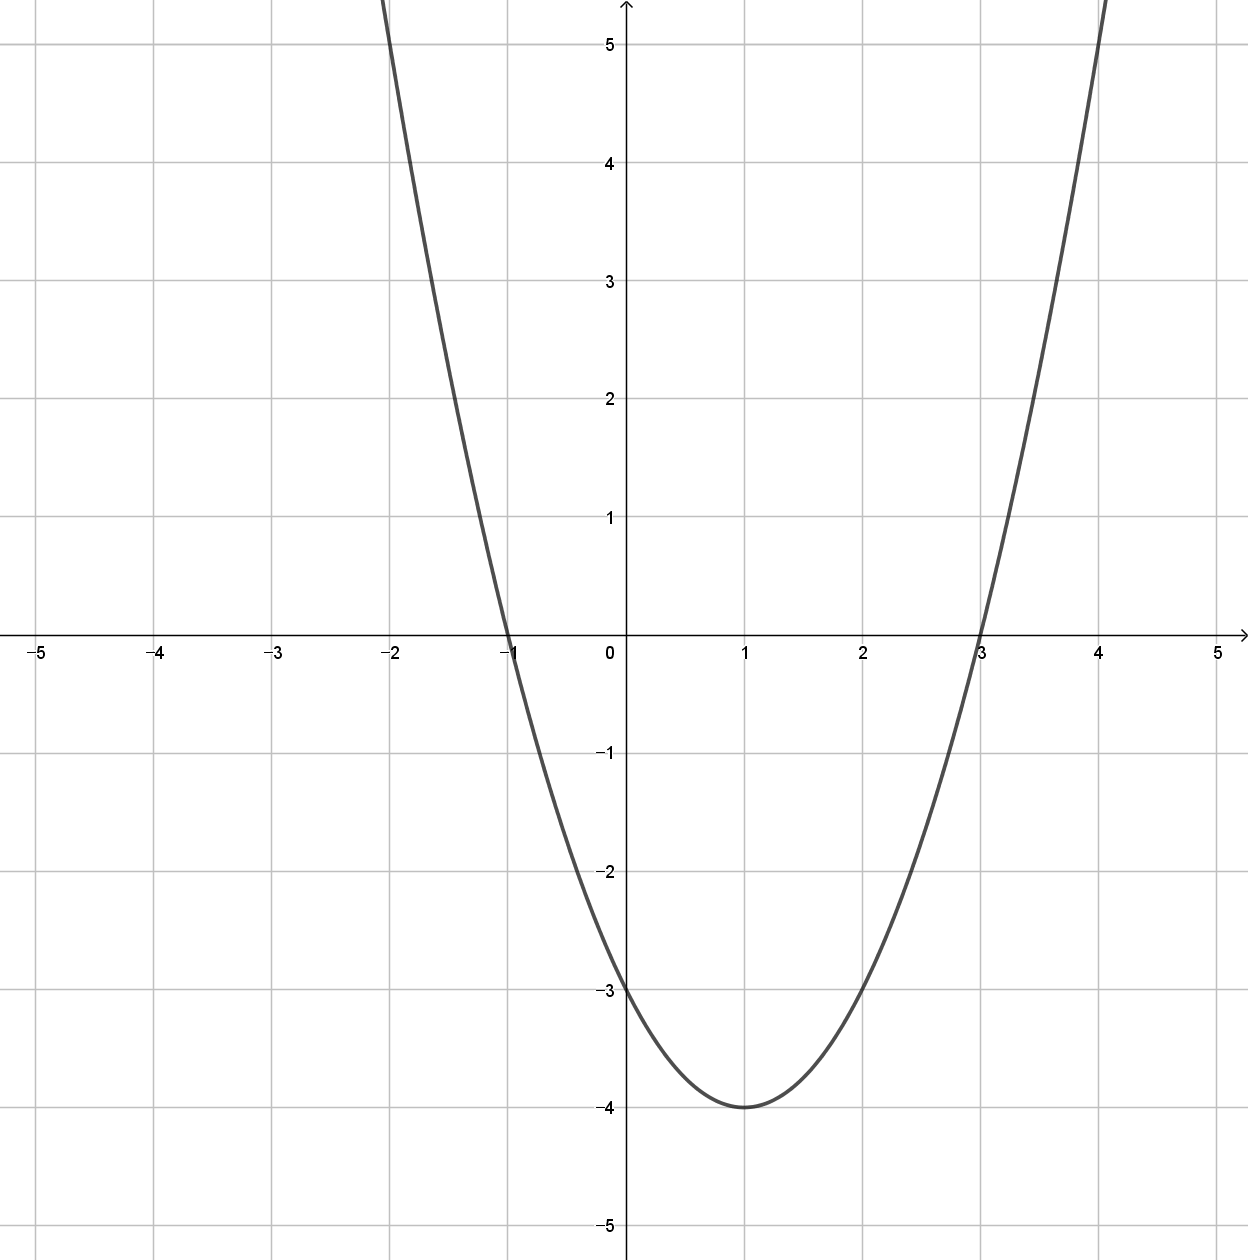
\includegraphics[width=0.5\textwidth]{y=x^2-2x-3}
\end{figure}

%
\exam{이차함수 \(y=x^2+3x+3\)의 그래프를 그리고\\ \ding{172}꼭짓점,\quad \ding{173}대칭축,\quad \ding{174} \(y\)절편,\quad \ding{175} \(x\)절편을 각각 구하여라.}
\begin{mdframed}[skipabove=-20pt]
\begin{enumerate}
\item[\ding{172}]
\begin{align*}
y
=&x^2+3x+3\\
=&x^2+3x+\frac94-\frac94+3\\
=&\left(x+\frac32\right)^2+\frac34\\
\end{align*}
에서 \(꼭짓점=\left(-\frac32,\frac34\right)\)이다.
\item[\ding{173}]
대칭축은 \(x=-\frac32\)이다.
\item[\ding{174}]
\(x=0\)을 대입하면 \(y=0^2+3\cdot0+3=3\)이므로 \(y\)절편은 \(3\)이다..
\item[\ding{175}]
\(y=0\)을 대입하면 \(0=x^2+3x+3\)에서 \(D=3^2-4\cdot1\cdot3=-3<0\)이므로 \(x\)절편은 없다.
\end{enumerate}
\end{mdframed}

\begin{figure}[h!]
\centering
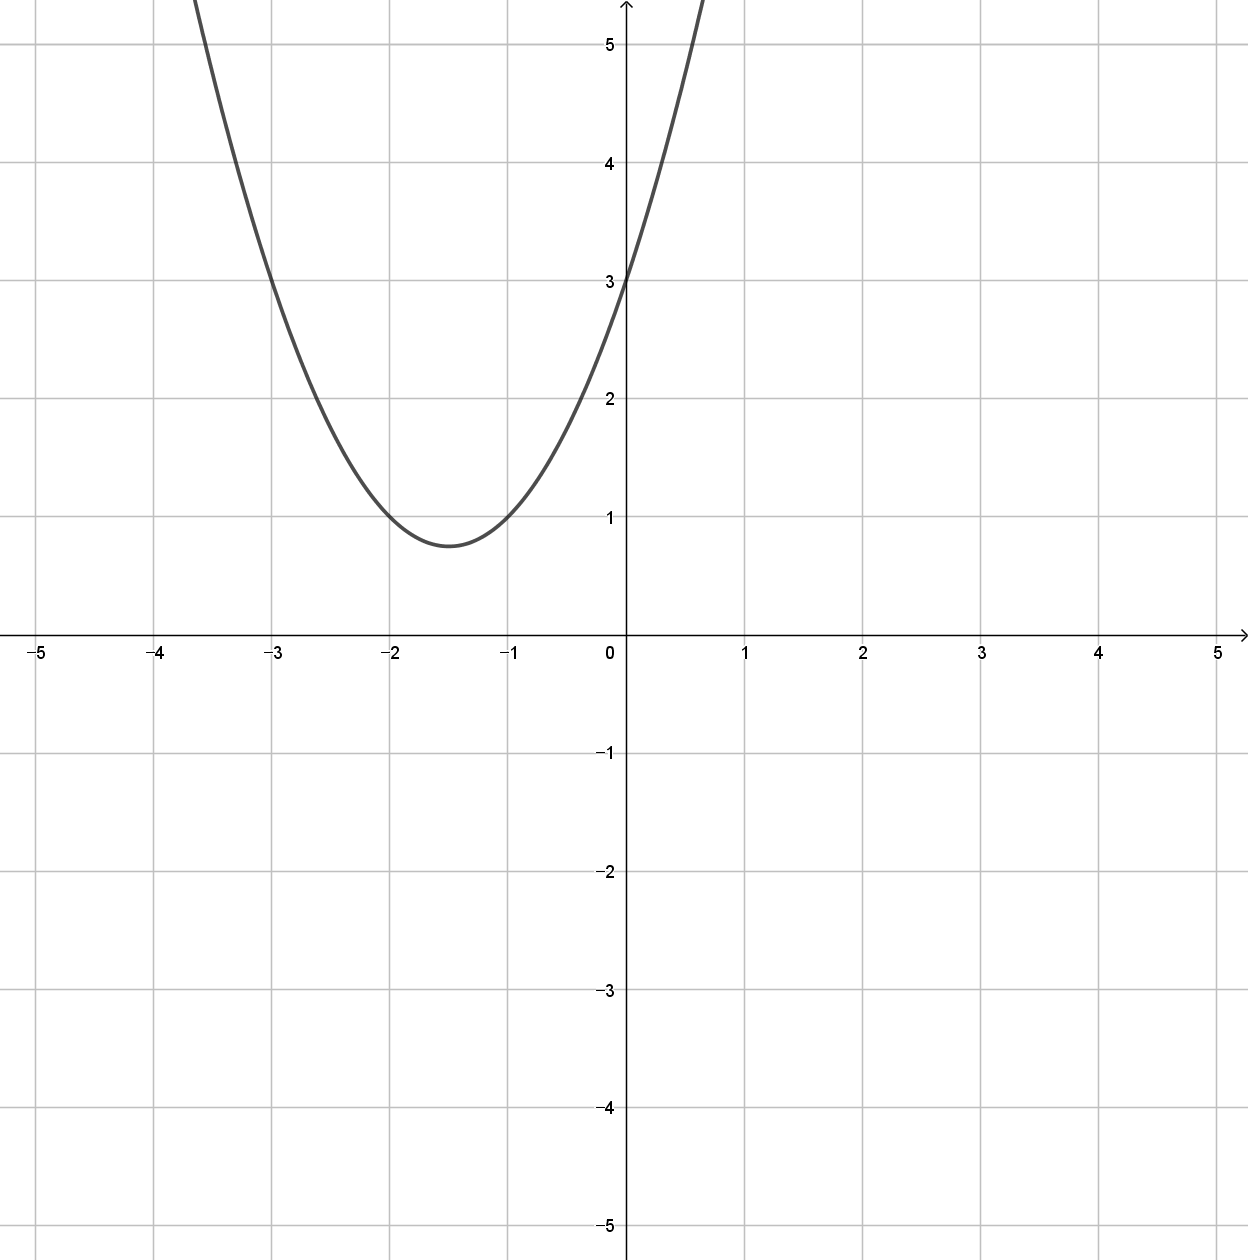
\includegraphics[width=0.5\textwidth]{y=x^2+3x+3}
\end{figure}

\clearpage
%
\prob{다음 이차함수들의 그래프를 그리고\\ \ding{172}꼭짓점,\quad \ding{173}대칭축,\quad \ding{174} \(y\)절편,\quad \ding{175} \(x\)절편을 각각 구하여라.}
\begin{enumerate}\label{grap1}
\item
\(y=-x^2+4x\)
\item
\(y=2x^2-2x+1\)
\end{enumerate}
\begin{mdframed}
\begin{enumerate}
\item
\item
\vspace{0.3\textwidth}
\end{enumerate}
\vspace{0.3\textwidth}
\end{mdframed}
\begin{minipage}{0.49\textwidth}\centering
\par\bigskip\includegraphics[width=0.9\textwidth]{55}
\end{minipage}
\begin{minipage}{0.49\textwidth}\centering
\par\bigskip\includegraphics[width=0.9\textwidth]{55}
\end{minipage}\bigskip\bigskip\par

%%
\subsection{그래프의 위치관계}
이차함수 \(y=ax^2+bx+c\)의 \(x\)절편을 구하려면 \(y=0\)을 대입해
\[ax^2+bx+c=0\]
을 풀어서 얻는다.
따라서 이차함수의 그래프와 \(x\)축의 교점의 개수는 이 이차방정식의 근의 개수와 관련이 있다.

\bigskip\noindent
\begin{tabu}{X[1,c]|X[2,c]|X[2,c]|X[2,c]}
\hline
&\(D>0\)		&\(D=0\)	&\(D<0\)\\
\hline
\(a>0\)
&\raisebox{-.5\height}{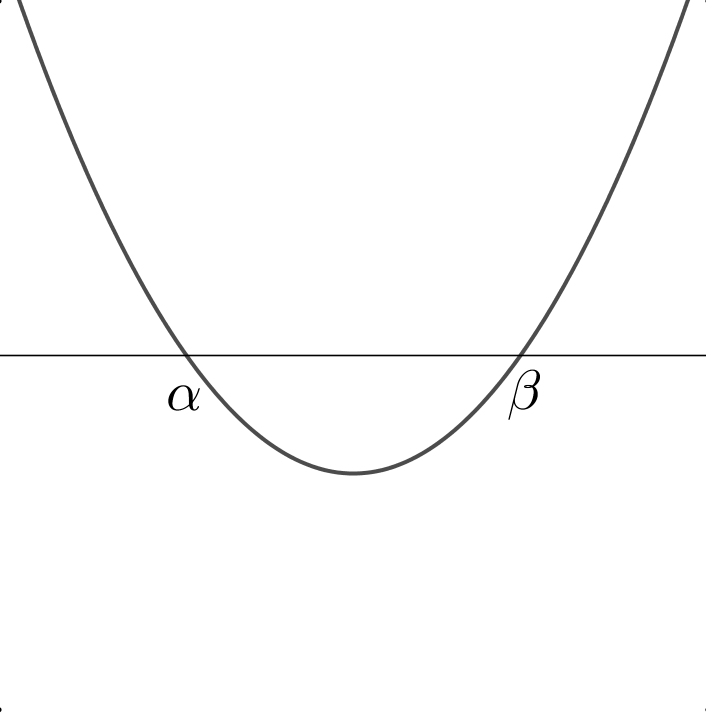
\includegraphics[width=0.24\textwidth]{1}}
&\raisebox{-.5\height}{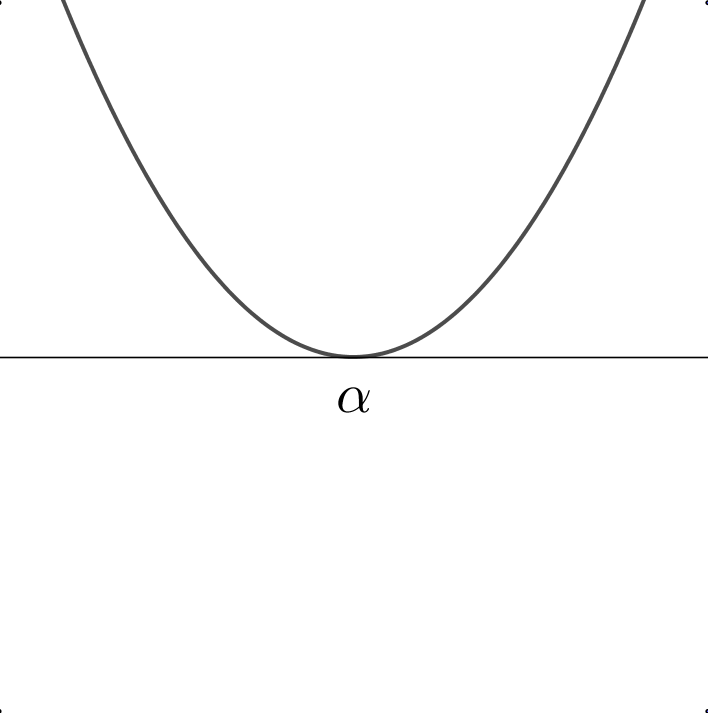
\includegraphics[width=0.24\textwidth]{2}}
&\raisebox{-.5\height}{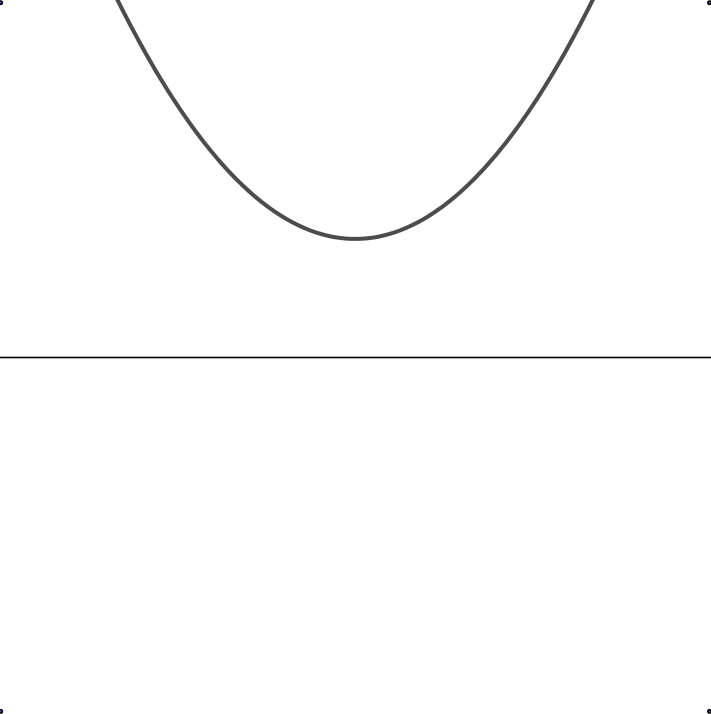
\includegraphics[width=0.24\textwidth]{3}}
\\\hline
\(a<0\)
&\raisebox{-.5\height}{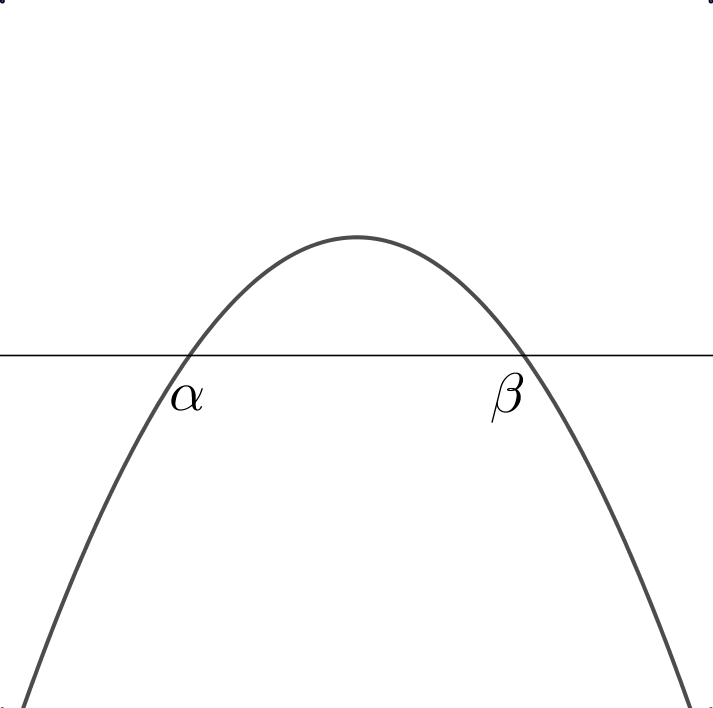
\includegraphics[width=0.24\textwidth]{4}}
&\raisebox{-.5\height}{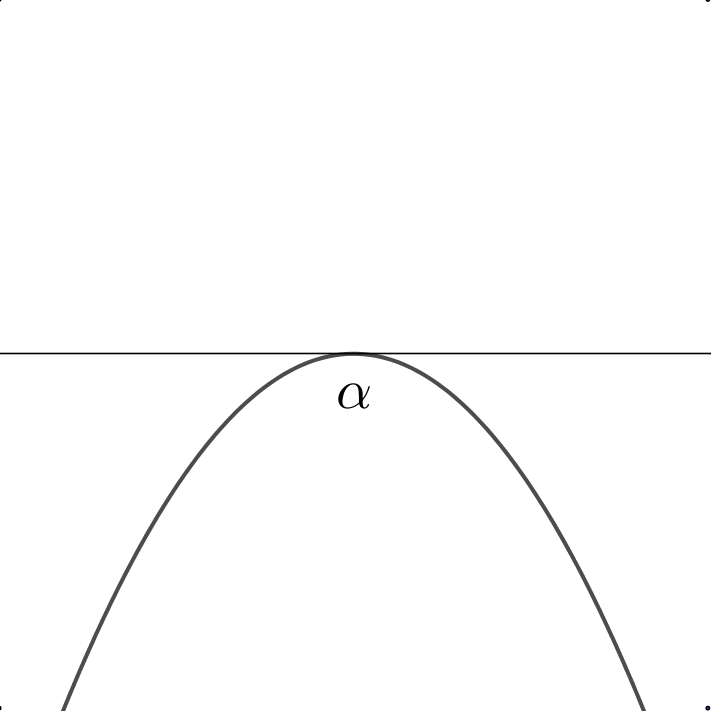
\includegraphics[width=0.24\textwidth]{5}}
&\raisebox{-.5\height}{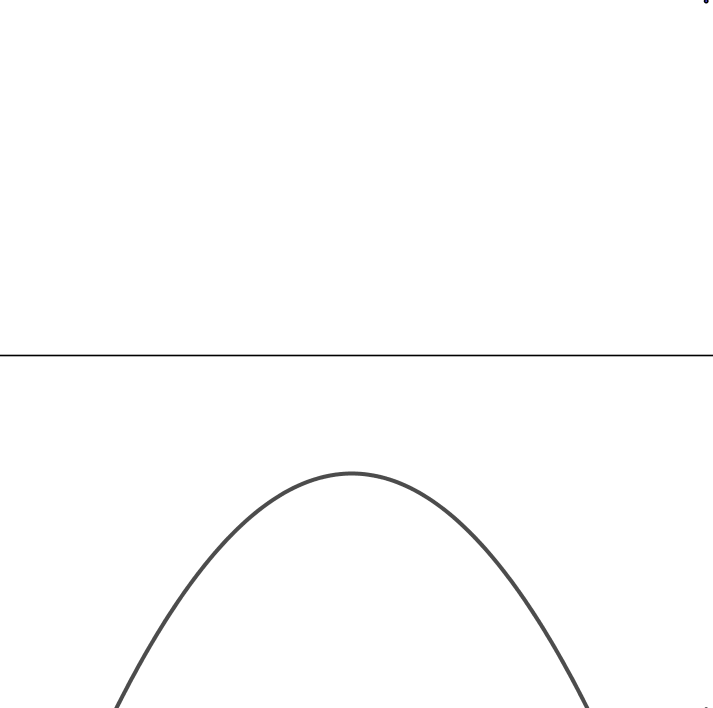
\includegraphics[width=0.24\textwidth]{6}}
\\\hline
\rowfont{\footnotesize}
교점의 개수&2개&1개&0개
\\\hline
\end{tabu}

%
\exam{다음 이차함수의 그래프와 \(x\)축의 위치 관계를 말하여라.}
(1) \(y=x^2-3x+1\)
\tabto{0.5\textwidth}
(2) \(y=-2x^2-2x-1\)
\begin{mdframed}
\begin{enumerate}
\item
\(D=(-3)^2-4\cdot1\cdot1=5>0\)이므로\\
이차함수의 그래프는 \(x\)축과 두 점에서 만난다.
\item
\(D/4=(-1)^2-(-2)(-1)=-1<0\)이므로\\
이차함수의 그래프는 \(x\)축과 만나지 않는다.
\end{enumerate}
\end{mdframed}

\clearpage
%
\exam{}
두 함수 \(y=x^2-4x+2,\quad y=x-2\)의 그래프의 교점의 좌표를 구하여라.
\begin{mdframed}
두 함수의 교점 \((x,y)\)는 두 식을 모두 만족시킨다.
따라서 연립방정식
\[\begin{cases}y=x^2-4x+2\\y=x-2\end{cases}\]
을 풀면 교점의 좌표를 얻을 수 있다.
\(y\)를 소거해 \(x\)를 구하면
\begin{gather*}
x^2-4x+2=x-2\\
x^2-5x+4=0\\
(x-1)(x-4)=0\\
x=1\text{ 또는 }x=4
\end{gather*}
\(x=1\)이면 \(y=-1\)이고 \(x=4\)이면 \(y=2\)이므로
두 그래프의 교점의 좌표는 \((1,-1)\)과 \((4,2)\)이다.
\end{mdframed}
\begin{figure}[h!]
\centering
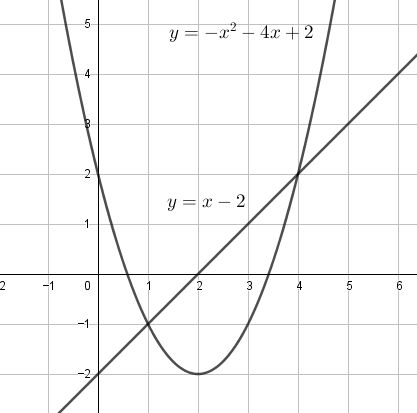
\includegraphics[height=0.3\textheight]{intersects}
\end{figure}

%
\prob{다음 함수들의 그래프의 교점의 좌표를 구하여라.}
\begin{enumerate}\label{grap2}
\item
\(y=-x^2+3x,\quad y=-2x+4\)
\item
\(y=x^2+2,\quad y=2x+1\)
\end{enumerate}



%%%
\section*{답}
\addcontentsline{toc}{chapter}{\protect\numberline{*}답}
\begin{minipage}[t]{0.49\textwidth}
%
\an{comp2}
(1) \(x=\pm\sqrt3i\)\\
(2) \(x=\pm\frac12i\)\\
(3) \(x=-3\pm i\)

%
\an{comp3}
\(x=1\), \(y=3\), \(z=1\)

%
\an{comp4}
\ding{175}

%
\an{comp5}
(1) \(a=-4\), \(b=2\)\\
(2) \(a=1\), \(b=2\)

%
\an{comp6}
(1) \(3-2i\)\\
(2) \(4+i\)\\
(3) \(-8\)\\
(4) \(-15i\)

%
\an{comp7}
(1) \(b=0\)\\
(2) \(a=0\)
\end{minipage}
%%
\begin{minipage}[t]{0.49\textwidth}
%
\an{comp8}
(1) \(1+2i\)\\
(2) \(2\sqrt2i\)\\
(3) \(4+6i\)\\
(4) \(7-9i\)\\
(5) \(17\)\\
(6) \(1\)\\
(7) \(-1\)\\
(8) \(-27i\)

%
\an{comp9}
(1) 실수부분 : \(\frac12\), 허수부분 : \(-\frac12\)\\
(2) 실수부분 : \(0\), 허수부분 : \(-1\)\\
(3) 실수부분 : \(\frac5{13}\), 허수부분 : \(\frac{12}{13}\)\\

%
\an{comp10}
(1) \(5i\)\\
(2) \(\sqrt2i\)\\
(3) \(-i\)

%
\an{comp11}
\ding{174}

%
\an{line1}
\ding{174}

%
\an{quad1}
(1) \(x=\pm5\)\\
(2) \(x=\pm5i\)\\
(3) \(x=\pm\frac{\sqrt3}2i\)
\end{minipage}

\clearpage
%
\an{quad2}
\begin{mdframed}
(1) 인수분해를 이용한 풀이
\begin{gather*}
x^2-2x-8=0\\
(x-4)(x+2)=0\\
x=-2\quad또는\quad x=4
\end{gather*}
\end{mdframed}

\begin{mdframed}
(2) 완전제곱식을 이용한 풀이
\begin{gather*}
x^2-2x-8=0\\
x^2-2x=8\\
x^2-2x+1=8+1\\
(x-1)^2=9\\
x-1=\pm3\\
x=1\pm3
\end{gather*}
따라서 \(x=-2,\quad4\)
\end{mdframed}

\begin{mdframed}
(3) 근의 공식을 이용한 풀이\\
\(a=1\), \(b=-2\), \(c=-8\)에서
\[x=\frac{-b\pm\sqrt{b^2-4ac}}{2a}=\frac{-(-2)\pm\sqrt{(-2)^2-4\cdot1\cdot(-8)}}{2\cdot1}=\frac{2\pm6}{2}\]
따라서 \(x=-2,\quad4\)

혹은 \(b'=-1\)를 사용하여
\[x=\frac{-b'\pm\sqrt{b'^2-ac}}{a}=\frac{-(-1)\pm\sqrt{(-1)^2-1\cdot(-8)}}{1}=1\pm3\]
따라서 \(x=-2,\quad4\)
\end{mdframed}

\clearpage
%
\an{quad3}
\begin{mdframed}[skipabove=-30pt]
(2) 완전제곱식을 이용한 풀이
\begin{gather*}
3x^2+5x+1=0\\
x^2+\frac53x+\frac13=0\\
x^2+\frac53x=-\frac13\\[2ex]
x^2+\frac53x+\frac{25}{36}=\frac{25}{36}-\frac13\\[2ex]
\left(x+\frac56\right)^2=\frac{13}{36}\\[2ex]
x+\frac56=\pm\frac{\sqrt{13}}6\\[2ex]
x=-\frac56\pm\frac{\sqrt{13}}6
\end{gather*}
\end{mdframed}

\begin{mdframed}
(3) 근의 공식을 이용한 풀이\\
\(a=3\), \(b=5\), \(c=1\)에서
\[x=\frac{-b\pm\sqrt{b^2-4ac}}{2a}=\frac{-(-5)\pm\sqrt{(-5)^2-4\cdot3\cdot1}}{2\cdot3}=\frac{-5\pm\sqrt{13}}{6}\]
\end{mdframed}

%
\an{quad4}
\begin{mdframed}[skipabove=-30pt]
(2) 완전제곱식을 이용한 풀이
\begin{gather*}
x^2-6x+18=0\\
x^2-6x+9=-9\\
(x-3)^2=-9\\
x-3=\pm3i\\
x=3\pm3i
\end{gather*}
\end{mdframed}

\begin{mdframed}
(3) 근의 공식을 이용한 풀이\\
\(a=1\), \(b'=-3\), \(c=18\)에서
\[x=\frac{-b'\pm\sqrt{b'^2-ac}}{a}=\frac{-(-3)\pm\sqrt{(-3)^2-1\cdot18}}{1}
=3\pm3i\]
\end{mdframed}

\begin{minipage}{0.49\textwidth}
%
\an{quad5}
(1) 서로 다른 두 실근\\
(2) 서로 같은 두 실근(중근)\\
(3) 서로 다른 두 허근\\
(4) 서로 다른 두 허근

%
\an{quad6}
(1) 두 근의 합 : \(1\), 두 근의 곱 : \(3\)\\
(2) 두 근의 합 : \(3\), 두 근의 곱 : \(0\)\\
(3) 두 근의 합 : \(1\), 두 근의 곱 : \(-\frac52\)

%
\an{quad7}
(1) \(p=-8\), \(q=15\)\\
(2) \(p=-7\), \(q=2\)\\
(3) \(p=2\), \(q=-6\)

%
\an{grap1}
(1) \ding{172} \((2,4)\), \ding{173} \(x=2\), \ding{174} \(0\), \ding{175} \(0\), \(4\)\\
(2) \ding{172} \((\frac12,\frac12)\), \ding{173} \(x=\frac12\), \ding{174} \(1\), \ding{175} 없다.
\end{minipage}
%%
\begin{minipage}{0.49\textwidth}
\begin{center}
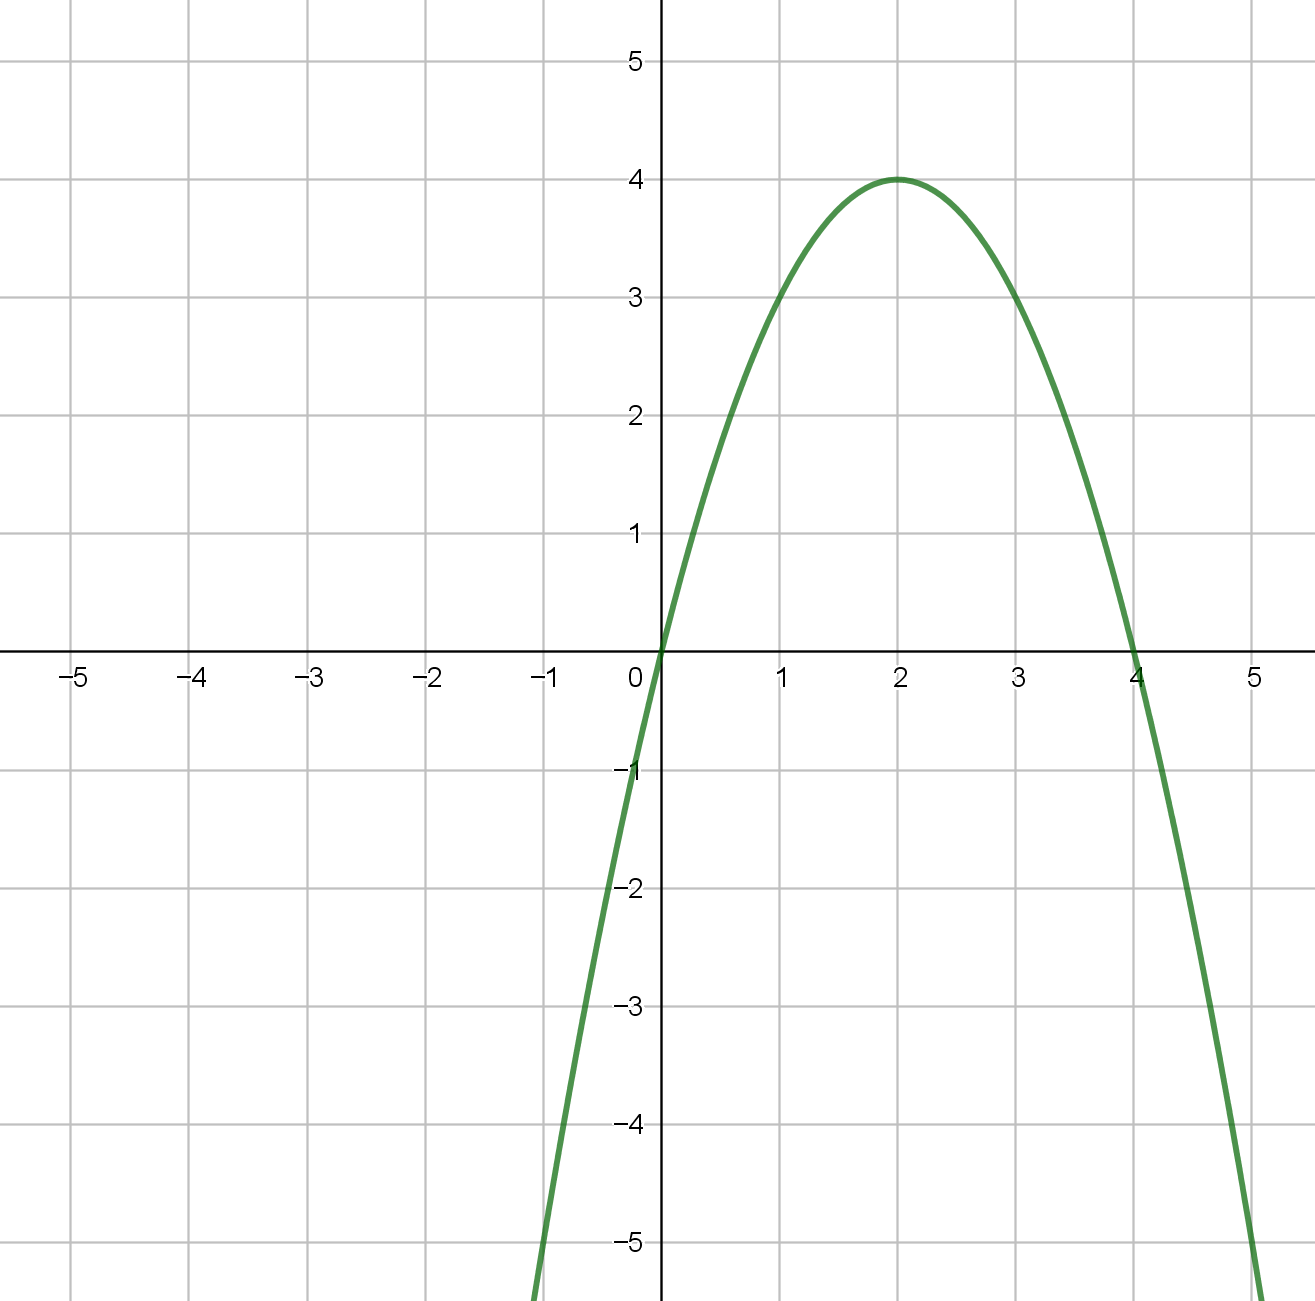
\includegraphics[width=0.9\textwidth]{y=-x^2+4x}
\par
(1)
\end{center}

\begin{center}
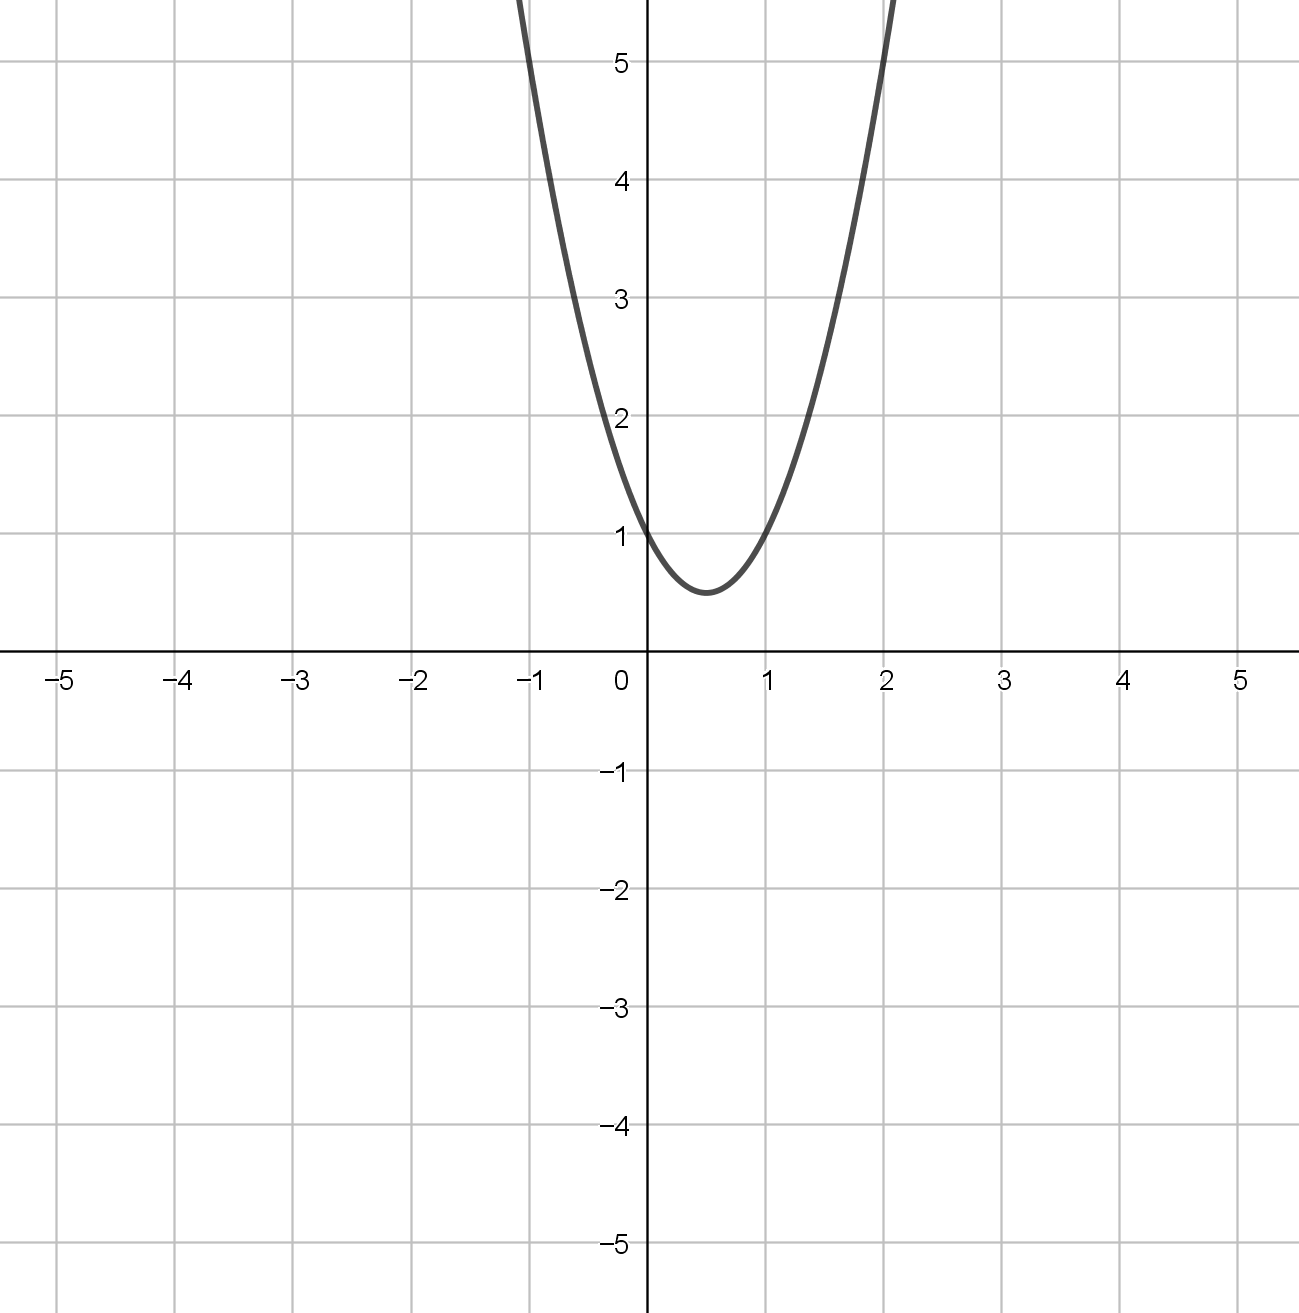
\includegraphics[width=0.9\textwidth]{y=2x^2-2x+1}
\par
(2)
\end{center}

%
\an{grap2}
(1) \((1,2)\), \((4,-4)\)\\
(2) \((1,3)\)
\end{minipage}
\end{document}